

\begin{center}
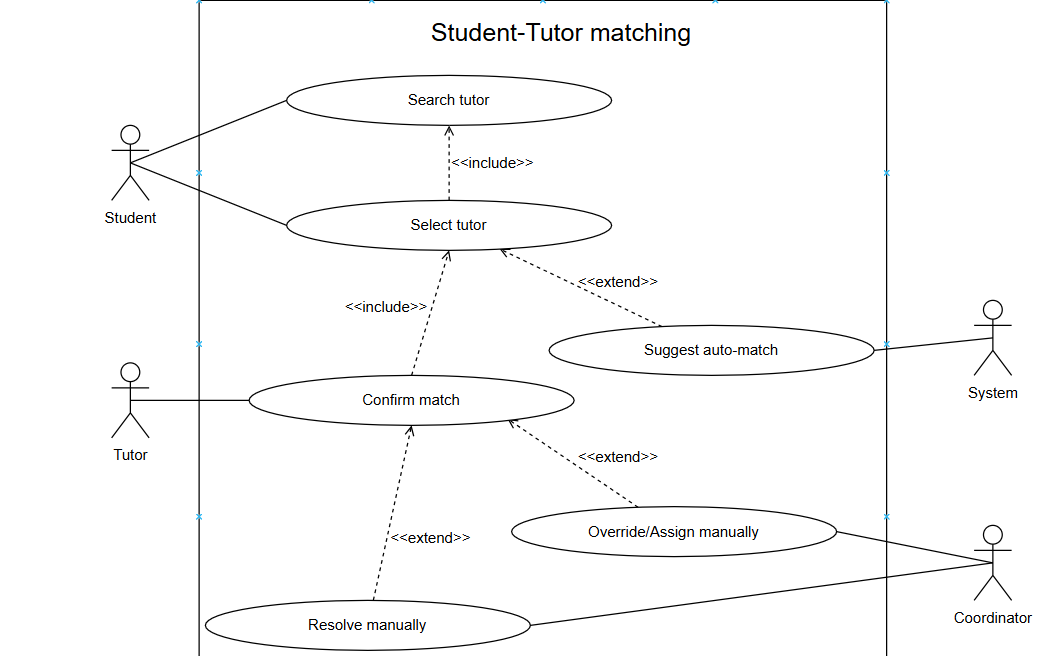
\includegraphics[width=0.9\linewidth]{images/UC-02.png}
\end{center}

\begin{center}
\textbf{Figure 3:}  Tutor--Student Matching
\end{center}

\begin{table}[h!]
\centering
\begin{tabular}{|p{3cm}|p{11cm}|}
\hline
\textbf{Use-case ID} & UC-02 \\
\hline
\textbf{Use-case name} & Tutor--Student Matching \\
\hline
\textbf{Use-case overview} & To allow students to search and select tutors manually or request an automated match, with tutor confirmation and coordinator intervention when necessary. \\
\hline
\textbf{Actors} & Student (primary), Tutor, Coordinator, System \\
\hline
\textbf{Preconditions} & 
1. Student and tutor profiles exist in the system. \newline
2. The system is operational and accessible. \newline
3. Student is authenticated in the system. \\
\hline
\textbf{Trigger} & Student initiates a search for tutors or requests an auto-match. \\
\hline
\textbf{Steps} &
1. Student searches for tutors by subject, availability, or preferences. \newline
2. Student selects a tutor; a pending match is created. \newline
3. System may suggest an auto-match (ranked list) based on the student's criteria. \newline
4. Tutor reviews the pending match and confirms the match. \newline
5. If confirmed, the system finalizes and logs the pairing. \\
\hline
\textbf{Postconditions} & A tutor--student pairing is established and logged in the system. \\
\hline
\textbf{Alternative Flows} & 
1. Auto-match rejected by student or tutor → Coordinator resolves manually. \newline
2. No tutors found → System suggests broadening search criteria. \newline
3. Tutor does not respond within time limit → Coordinator is notified to assign a tutor. \\
\hline
\textbf{Exception Flow} & 
1. Network failure prevents search or confirmation (system prompts user to retry). \newline
2. Tutor or student profile missing/corrupted → System logs an error and notifies Coordinator. \\
\hline
\end{tabular}
\caption{Use Case UC-02: Tutor--Student Matching}
\end{table}
